\documentclass[journal]{IEEEtran}
\usepackage[utf8]{inputenc}
\usepackage{amsmath,amssymb,graphicx,booktabs,url,balance}
\usepackage[hidelinks]{hyperref}
\usepackage{multirow}
\graphicspath{{figures/}}

\begin{document}

\title{CONCLAVE: Agentic AI Without a Language Model --- \\
Ensemble Machine Learning as the Cognitive Core for \\
Connectivity-Denied Autonomous Systems}

\author{Aranya~Mahmud%
\thanks{Department of Computer Science and Engineering, Daffodil International
University, Dhaka, Bangladesh. E-mail: aranyamahmud29@gmail.com}%
\thanks{Code, data-preparation scripts, and all result artefacts are available at
\url{https://github.com/<user>/conclave}.}}

\markboth{Preprint --- under review}%
{Mahmud: Agentic AI Without a Language Model}

\maketitle

\begin{abstract}
Every widely used agentic AI framework places a language model at the centre
of the sense--decide--act loop. That choice imports two dependencies that are
untenable in the environments where autonomy matters most: a network path to
a remote model, or enough local compute to host one. During a flood, a
cyclone, or an earthquake --- precisely when an autonomous responder is most
valuable --- cellular and backhaul infrastructure is among the first
casualties, and the field hardware that survives is battery-powered and
memory-constrained. We ask whether the language model is actually load-bearing
for the class of agentic tasks these deployments require, and find that it
often is not. We present \textbf{CONCLAVE}, a framework in which a heterogeneous
machine-learning ensemble replaces the language model as the cognitive core,
supplying action selection, open-vocabulary tool routing, calibrated
abstention, and an explicit uncertainty decomposition that a single model
cannot provide. On the Berkeley Function Calling Leaderboard, CONCLAVE's ranking
ensemble selects the correct tool with $90.8\%$ top-1 accuracy on the
user-contributed multi-tool split, $78.9\%$ when every test tool was unseen
during training, in $4.0$\,ms per decision from a $631$\,KB model. On the
HumAID crisis-triage benchmark it reaches $74.3\%$ weighted F1 against
$76.0\%$ for the RoBERTa baseline the dataset authors report on the same
combined split --- a $1.8$-point gap --- while exceeding every classical
baseline they report, from a $36$\,MB artefact rather than a $125$M-parameter
transformer. In
a sequential flood-response simulation, CONCLAVE is statistically
indistinguishable from an \emph{oracle} cloud agent under full connectivity
($\Delta = 0.6$, 95\% CI $[-0.7, 1.9]$) and significantly better once
outages begin, converting a $-127$ mean return into $+34$ when $73\%$ of
steps are offline. We also report a negative result: ensemble disagreement,
while an excellent detector of covariate shift (AUROC up to $0.955$), does
\emph{not} outperform random allocation when used to direct a scarce human
oversight budget in a sequential task. CONCLAVE is released under Apache-2.0.
\end{abstract}

\begin{IEEEkeywords}
Agentic AI, ensemble learning, edge computing, offline autonomy, disaster
response, uncertainty quantification, tool use.
\end{IEEEkeywords}

\section{Introduction}
\IEEEPARstart{T}{he} contemporary AI agent is defined by its cognitive core.
Frameworks such as LangGraph, CrewAI, AutoGen, and the various vendor agent
SDKs differ in orchestration, memory, and tooling, but agree on one point: a
large language model performs the reasoning, and everything else is
scaffolding. This consensus has proven productive for open-ended, text-mediated
work.

It is a poor fit for a distinct and important class of deployments. Consider a
flood-warning and response system in a riverine district. It ingests gauge
readings and radio traffic; it must decide when to broadcast a warning, when to
begin evacuation, when to commit scarce boats, and when to defer to a human
coordinator. The decisions recur with little variation, the input is largely
structured, and the consequences are severe. Crucially, the system's value peaks
exactly when the cellular network has failed. A cloud-backed agent in that
moment is not degraded; it is absent.

The field has recognised the resource half of this problem. A recent survey of
adaptive agentic AI for mobile and embedded devices~\cite{survey2025adaptive}
catalogues elastic inference, test-time adaptation, and cloud--edge offloading
--- but frames the entire design space around ``foundation models as the
cognitive core,'' so every technique is a way of \emph{compressing} the language
model. NVIDIA's position paper~\cite{belcak2025slm} pushes further, arguing that
because agentic invocations are ``a small number of specialised tasks performed
repetitively and with little variation,'' small language models are sufficient
and 10--30$\times$ cheaper. Empirical follow-up is sobering: TinyLLM's
evaluation of sub-3B models on function calling reports a best overall accuracy
of $65.74\%$~\cite{haque2025tinyllm}, and even a quantised 0.5B model needs
roughly half a gigabyte of weights.

We take the NVIDIA argument one step further than its authors do. If the task is
genuinely specialised, repetitive, and low-variance, the question is not how
small the language model can be --- it is whether a language model is required
at all. Natural language is a means of \emph{specifying} the task, not
necessarily of executing it. Once the tool set is registered and the decision
space is enumerated, the residual problem is classification, ranking, and
sequential control under uncertainty: the problem classical machine learning was
built for, and solves in kilobytes and microseconds.

This paper makes that case concretely.

\subsection{Contributions}
\begin{enumerate}
\item \textbf{A framework.} CONCLAVE realises the full agentic loop --- perception,
      action selection, open-vocabulary tool routing, symbolic planning over
      tool preconditions, case-based episodic memory, and hard safety
      constraints --- with a heterogeneous ML ensemble in place of a language
      model. It has no network dependency, requires no GPU, and serialises to
      under $250$\,KB for the disaster agent.
\item \textbf{Uncertainty as control flow.} Because the core is a committee,
      total predictive uncertainty decomposes into aleatoric and epistemic
      parts at no additional cost. CONCLAVE routes on this decomposition: act,
      gather more evidence, abstain, or escalate. We calibrate the thresholds
      by selective prediction rather than hand-tuning them.
\item \textbf{Bounded worst-case decision latency.} A decision is a fixed number
      of estimator evaluations and a bounded-depth planning search. There is no
      analogue of an unbounded generation loop, so p99 latency is a measurable
      constant --- a property that matters for certifying safety-critical
      autonomy.
\item \textbf{Evaluation across four axes,} on public benchmarks: tool routing
      and abstention (BFCL v3), crisis perception (HumAID), sequential control
      under connectivity loss, and resource cost under emulated edge profiles.
\item \textbf{An honest negative result.} We show where the approach's central
      intuition fails: instantaneous ensemble disagreement is a poor allocator
      of scarce human oversight in sequential tasks, losing to random
      allocation. We analyse why and identify the correction.
\end{enumerate}

\section{Related Work}

\subsection{LLM-centred agent frameworks}
The dominant frameworks all assume a language model performs reasoning, tool
selection, and planning. Their limitations under resource constraint are
well-documented and have prompted an active compression literature, but the
architectural assumption is rarely questioned. Work on LLM planning
competence~\cite{kambhampati2023selfcritique} independently suggests that
autoregressive models are weak planners absent an external verifier, which
further undercuts the case for placing one at the centre of a control loop.

\subsection{Small language models at the edge}
The SLM-agent line~\cite{belcak2025slm,haque2025tinyllm} shares our diagnosis ---
that agentic workloads are narrow and repetitive --- but not our conclusion.
TinyLLM~\cite{haque2025tinyllm} is our closest point of comparison: it evaluates
TinyAgent, TinyLlama, Qwen, and xLAM on BFCL with SFT, PEFT, RL, and DPO
optimisation, reaching $65.74\%$ overall and $55.62\%$ multi-turn accuracy. We
note carefully that BFCL's headline metric includes argument-level AST matching,
so our tool-selection numbers are \emph{not} directly comparable; we make the
comparison only on cost, where the gap is several orders of magnitude, and on
the routing sub-task, which we measure separately.

\subsection{Agentic AI for disaster management}
Disaster Copilot~\cite{li2025disastercopilot} proposes a multi-agent
orchestrator for disaster response and explicitly raises resource-limited
operation, but it is a vision paper: no implementation, and on-device
orchestration is a design goal rather than a measured result. Deployed AIoT
flood systems typically use a fixed model pipeline with no agency --- no tool
selection, no abstention, no planning. CONCLAVE occupies the space between: real
autonomy, actually offline.

\subsection{Ensembles and uncertainty}
That ensembles improve accuracy and produce useful uncertainty estimates is
long established~\cite{dietterich2000ensemble,breiman2001randomforest,%
lakshminarayanan2017deepensembles}. The mutual-information decomposition we use
originates in Bayesian active learning~\cite{houlsby2011bald}, and selective
prediction has its own literature~\cite{elyaniv2010selective,%
geifman2017selectivenet}. Our contribution is not these components but their
composition: using them as the \emph{control substrate} of an autonomous agent,
and evaluating whether that composition survives contact with agentic
benchmarks.

\section{The CONCLAVE Framework}

\subsection{Overview}
An CONCLAVE tick is:
\[
\text{observe} \rightarrow \text{featurise} \rightarrow
\underbrace{\text{ensemble posterior}}_{\text{committee}} \rightarrow
\underbrace{\text{episodic prior}}_{\text{k-NN}} \rightarrow
\text{gate} \rightarrow \text{constraints} \rightarrow \text{act}
\]
Every stage is a bounded amount of arithmetic and none touches the network.

\subsection{Observations and budgeted features}
An \texttt{Observation} carries numeric features (gauge readings, resource
counts) and optional free text (a radio transcript, an SMS field report).
Text is featurised by the hashing trick with TF--IDF reweighting, so the
featuriser has \emph{no stored vocabulary} and its footprint is fixed at
construction. This is the single most consequential engineering choice for
microcontroller-class targets: a conventional fitted vocabulary on HumAID
occupies roughly $98$\,MB, whereas the hashed featuriser is constant-size and
tunable by one parameter, which we sweep in Section~\ref{sec:humaid}.

\subsection{The ensemble brain}
The core is a soft-voting committee of \emph{deliberately heterogeneous}
members --- a boosted tree model, a bagged forest, and a linear
model, plus a generative naive-Bayes member for text. Homogeneity is the
failure mode to avoid: a random forest's trees share an inductive bias, so
their disagreement collapses off-distribution exactly when the agent most
needs a warning. Mixing model families keeps the disagreement signal alive.

Two defaults are set from measurement rather than convention. First,
\texttt{n\_jobs=1}: an agent decides about one observation at a time over a
handful of candidate actions, and joblib's thread-pool construction costs
roughly $20\times$ more than the prediction itself at that batch size
($90$\,ms versus $4$\,ms in our measurements). Parallelism is a throughput
optimisation and a latency pessimisation; edge agents want the latter. Second,
shallow forests: depth-10, 60-estimator forests lose well under a point of
accuracy against unbounded 200-tree forests while cutting the serialised model
roughly $9\times$.

\subsection{Uncertainty decomposition as control flow}
For member posteriors $\{p_m\}_{m=1}^{M}$ over $K$ actions with mean
$\bar{p}$, we compute
\begin{align}
\underbrace{\mathcal{H}[\bar{p}]}_{\text{total}} =
\underbrace{\tfrac{1}{M}\textstyle\sum_m \mathcal{H}[p_m]}_{\text{aleatoric}} +
\underbrace{\Big(\mathcal{H}[\bar{p}] - \tfrac{1}{M}\textstyle\sum_m
\mathcal{H}[p_m]\Big)}_{\text{epistemic}},
\end{align}
each normalised by $\log K$. The distinction is operationally meaningful. High
aleatoric uncertainty means the members agree the situation is genuinely
ambiguous; more sensing will not help, so the agent should abstain. High
epistemic uncertainty means the members disagree --- the agent is outside its
competence, and should gather evidence or escalate. A single model cannot
separate these without expensive sampling; a committee gets it for free.

Gate thresholds are \emph{calibrated}, not chosen: we select the largest
coverage whose accuracy on accepted decisions meets a target precision, which
is standard selective prediction and keeps the framework honest.

\subsection{Open-vocabulary tool routing}
Rather than classifying into a fixed action label set, the router scores
\emph{(request, tool-specification) pairs} with a ranking ensemble over
lexical-overlap, TF--IDF-similarity, and schema-structure features. Because it
scores pairs, a tool registered after training is scored by the same features
as any other --- the agent gains capabilities without retraining, which is the
property that makes LLM routers attractive in the first place. Specification
vectors are static and cached at registration, so routing costs one query
vectorisation plus a few sparse dot products.

\subsection{Planning, memory, and constraints}
A cost-optimal forward search over tool preconditions and effects, with an
admissible set-cover heuristic and a hard depth bound, handles action ordering;
termination is guaranteed by construction. Episodic memory is a capacity-bounded
$k$-NN store over past (observation, action, reward) cases that contributes a
prior over actions --- the ensemble agent's counterpart to in-context learning,
at kilobytes and microseconds. Finally, a constraint layer sits \emph{above} the
learned policy: no statistical model may authorise an irreversible act on its
own, and a violated constraint converts the action into a recorded escalation.

\section{Experimental Setup}
All experiments run on a 2-core x86\_64 Linux container with $3.82$\,GB RAM
--- itself close to a Raspberry Pi profile --- with seeds fixed at $42$ and full
provenance recorded in every result artefact. Software: scikit-learn
$1.7.2$~\cite{pedregosa2011sklearn}, LightGBM $4.7.0$~\cite{ke2017lightgbm},
NumPy $2.2.6$.

\begin{table}[t]
\centering
\caption{Benchmarks and what each isolates.}
\label{tab:datasets}
\small
\begin{tabular}{@{}lll@{}}
\toprule
Benchmark & Size & Capability isolated \\
\midrule
BFCL v3~\cite{patil2024bfcl}   & 1{,}700 functions & tool routing, abstention \\
HumAID~\cite{alam2021humaid}   & 76{,}484 tweets   & crisis perception \\
Flood-response sim             & 40-step episodes  & sequential control \\
Edge profiles                  & 5 boards          & resource cost \\
\bottomrule
\end{tabular}
\end{table}

We note one discarded dataset, because the reason generalises. A widely-used
Bangladesh flood-prediction dataset gives $99.6\%$ accuracy under a standard
ensemble --- but a depth-1 decision stump on rainfall alone scores $98.4\%$,
and $92\%$ of rows are positive. Its ``Flood?'' label is essentially a rainfall
threshold, so any model recovers it and the benchmark measures nothing. We
report this because such labels are common in applied disaster-ML papers and
are rarely audited.

\section{Results}

\subsection{Tool routing and abstention}
\begin{table}[t]
\centering
\caption{Tool routing on BFCL v3. Latency is per single decision, not
amortised over a batch.}
\label{tab:routing}
\small
\begin{tabular}{@{}lrrrr@{}}
\toprule
Split & $n$ & Lexical & \textbf{CONCLAVE} & ms/dec. \\
\midrule
\texttt{multiple}            & 60  & 90.0\% & \textbf{98.3\%} & 4.72 \\
\texttt{live\_multiple}      & 316 & 79.4\% & \textbf{90.8\%} & 3.99 \\
\texttt{live\_multiple} (unseen tools) & 346 & 56.7\% & \textbf{78.9\%} & 4.35 \\
\midrule
Abstention (irrelevance)     & 2{,}628 & --- & 84.3\% acc / 0.921 AUC & 0.11 \\
\bottomrule
\end{tabular}
\end{table}

Table~\ref{tab:routing} and Fig.~\ref{fig:routing} report the results. The
ranking ensemble reaches $90.8\%$ top-1 accuracy on the user-contributed
multi-tool split at $3.99$\,ms per decision (p99 $7.09$\,ms) from a $631$\,KB
model. The lexical-similarity control isolates how much comes from learning:
$11.4$ points on the standard split, and $22.2$ points on the unseen-tool
split, where the router still reaches $78.9\%$ on tools absent from training.
Abstention --- deciding no tool applies --- reaches $0.921$ AUC at $0.11$\,ms.

For context, TinyLLM~\cite{haque2025tinyllm} reports $65.74\%$ overall BFCL
accuracy for optimised sub-3B models. We stress that this is a different
metric, including argument-level matching, and we do not claim to beat it. The
defensible comparison is cost: three orders of magnitude in model size, and
milliseconds against the hundreds of milliseconds to seconds an SLM needs per
generation on ARM hardware.

\begin{figure}[t]
\centering
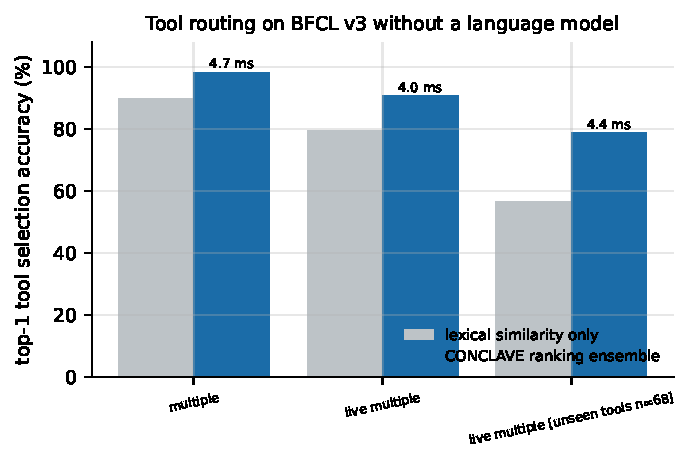
\includegraphics[width=\columnwidth]{fig5_routing.pdf}
\caption{Tool routing on BFCL v3. Learning contributes 11--22 points over
lexical matching, with the largest gain where tools were unseen in training.}
\label{fig:routing}
\end{figure}

\subsection{Crisis perception}
\label{sec:humaid}
\begin{table}[t]
\centering
\caption{HumAID triage, combined 10-class split. Baselines are as reported by
the dataset authors~\cite{alam2021humaid}, Table 7, row ``All''. The feature
budget is CONCLAVE's deployment knob.}
\label{tab:humaid}
\small
\begin{tabular}{@{}lrrr@{}}
\toprule
Model & Weighted F1 & Size & ms/dec. \\
\midrule
\multicolumn{4}{@{}l}{\emph{Reported by the dataset authors}} \\
RoBERTa            & \textbf{0.760} & $\sim$500\,MB & --- \\
BERT / DistilBERT / XLM-R & 0.758 & 250--500\,MB & --- \\
FastText           & 0.744 & --- & --- \\
SVM                & 0.731 & --- & --- \\
Random Forest      & 0.707 & --- & --- \\
\midrule
\multicolumn{4}{@{}l}{\emph{This work}} \\
CONCLAVE $2^{16}$ features & 0.743 & 36.4\,MB & 4.94 \\
CONCLAVE $2^{14}$ features & 0.726 & 10.1\,MB & 1.82 \\
CONCLAVE $2^{12}$ features & 0.713 & \textbf{2.6\,MB} & \textbf{1.27} \\
\bottomrule
\end{tabular}
\end{table}

Table~\ref{tab:humaid} and Fig.~\ref{fig:frontier} give the accuracy--footprint
frontier on the authors' combined split. CONCLAVE lands $1.8$ weighted-F1 points
behind RoBERTa using a $14\times$ smaller artefact, and matches FastText
($0.743$ vs $0.744$) while clearly exceeding the authors' SVM ($0.731$) and
random forest ($0.707$). Even the $2.6$\,MB configuration ($0.713$) edges past
their random forest --- at a size where a transformer is simply not an option.
We do not claim to match RoBERTa; we claim the trade is favourable when the
alternative is no agent at all.

One caution for readers comparing against this dataset: Table 7
of~\cite{alam2021humaid} also contains a column average of $0.781$, computed
across per-event and event-type rows. It is not the combined-dataset result and
should not be used as the baseline for work evaluated on the combined split, as
we initially did before checking the source table.

\begin{figure}[t]
\centering
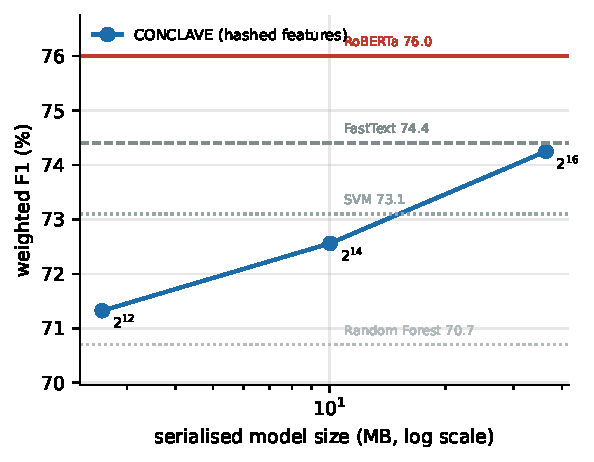
\includegraphics[width=0.82\columnwidth]{fig2_frontier.pdf}
\caption{Accuracy against deployment footprint on HumAID. Each point is a
hashed-feature budget.}
\label{fig:frontier}
\end{figure}

\subsection{Sequential control under connectivity loss}
This is the experiment the work exists for, and it is deliberately stacked
against us. The cloud baseline runs an \textbf{oracle} policy with access to
the simulator's latent risk --- no real language model would do this well.
CONCLAVE sees only noisy sensors and a text field report, and was trained by
behaviour cloning on that same expert, so it is strictly weaker in capability.
Any advantage therefore comes from availability alone.

\begin{table}[t]
\centering
\caption{Mean episode return under connectivity loss, 120 episodes per cell.
Paired bootstrap over identical episode seeds.}
\label{tab:availability}
\small
\begin{tabular}{@{}rrrrl@{}}
\toprule
Offline & \textbf{CONCLAVE} & Cloud oracle & $\Delta$ & 95\% CI \\
\midrule
0.0\%  & $36.5$ & $35.8$   & $+0.6$   & $[-0.7,\ 1.9]$ \\
35.3\% & $33.9$ & $-34.2$  & $+68.1$  & $[57.6,\ 78.9]$ \\
53.0\% & $34.3$ & $-77.7$  & $+112.0$ & $[100.6,\ 123.6]$ \\
62.3\% & $34.8$ & $-99.3$  & $+134.2$ & $[122.9,\ 145.8]$ \\
68.6\% & $34.9$ & $-113.2$ & $+148.1$ & $[136.2,\ 160.3]$ \\
73.1\% & $33.5$ & $-127.3$ & $+160.8$ & $[148.5,\ 173.0]$ \\
\bottomrule
\end{tabular}
\end{table}

Table~\ref{tab:availability} and Fig.~\ref{fig:availability} show the result.
Under full connectivity the two are statistically indistinguishable
($\Delta = 0.6$, CI $[-0.7, 1.9]$), which confirms behaviour cloning recovered
the expert and validates the comparison as fair. From the first outage regime
onward, CONCLAVE is significantly better, and the gap widens monotonically. In
casualty terms, the oracle agent's mean rises from $53.7$ to $276.9$ as
connectivity degrades, while CONCLAVE stays between $41.9$ and $50.0$. A
last-action cache recovers roughly half the loss but no more: stale actions in
a fast-moving flood are only marginally better than none. Static threshold
rules --- the real-world incumbent --- are unaffected by outages, as expected,
but are far worse than either agent throughout.

\begin{figure}[t]
\centering
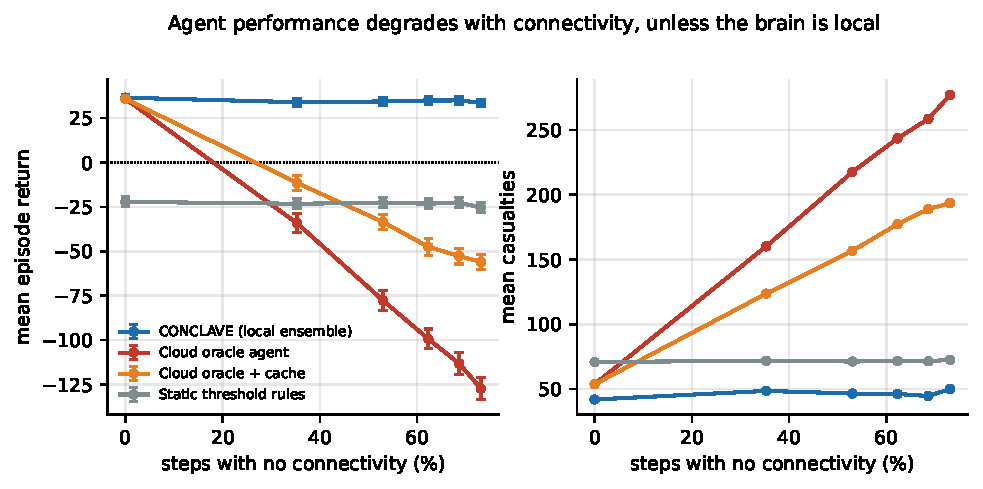
\includegraphics[width=\columnwidth]{fig1_availability.pdf}
\caption{Return and casualties against measured offline fraction. The cloud
agent has an oracle policy; its collapse is availability, not capability.}
\label{fig:availability}
\end{figure}

\subsection{Resource cost}
\begin{table}[t]
\centering
\caption{Decision cost under emulated edge profiles. Measured values were
obtained with the board's core count and an enforced RAM ceiling; on-device
columns are estimates scaled by relative single-core throughput.}
\label{tab:edge}
\small
\begin{tabular}{@{}lrrrr@{}}
\toprule
& \multicolumn{2}{c}{Measured (host)} & \multicolumn{2}{c}{Estimated on-device} \\
\cmidrule(lr){2-3}\cmidrule(lr){4-5}
Board & mean & p99 & mean & energy \\
\midrule
Host (2-core x86) & 2.47\,ms & 3.07\,ms & 2.47\,ms & 37.1\,mJ \\
Jetson Nano       & 2.46\,ms & 3.23\,ms & 9.47\,ms & 94.7\,mJ \\
Raspberry Pi 4B   & 2.44\,ms & 3.64\,ms & 8.72\,ms & 55.8\,mJ \\
Raspberry Pi 3B+  & 2.43\,ms & 2.87\,ms & 14.27\,ms & 71.4\,mJ \\
Pi Zero 2 W       & 2.49\,ms & 3.37\,ms & 22.59\,ms & 56.5\,mJ \\
\bottomrule
\end{tabular}
\end{table}

Each cell is the lowest-median batch of five independent batches of 120
decisions. Interference from other processes can only make a timing slower, so
a single batch is an upper bound contaminated by whatever else the machine was
doing; taking the quietest batch is the least-contaminated estimate. We also
record the ratio of worst to best batch median (at most $1.19$ here) so that
contamination stays visible rather than being averaged away. Without this, we
measured p99 figures that varied by $2.5\times$ between runs on the same code.

We separate measurement from modelling, because conflating them is how resource
claims fail review. Measured: single-decision latency with the target's core
count and an enforced \texttt{RLIMIT\_AS} ceiling, peak resident memory, and
serialised size. Estimated, and labelled as such: on-device latency scaled by
relative single-core throughput, and energy as latency $\times$ TDP.

\begin{figure}[t]
\centering
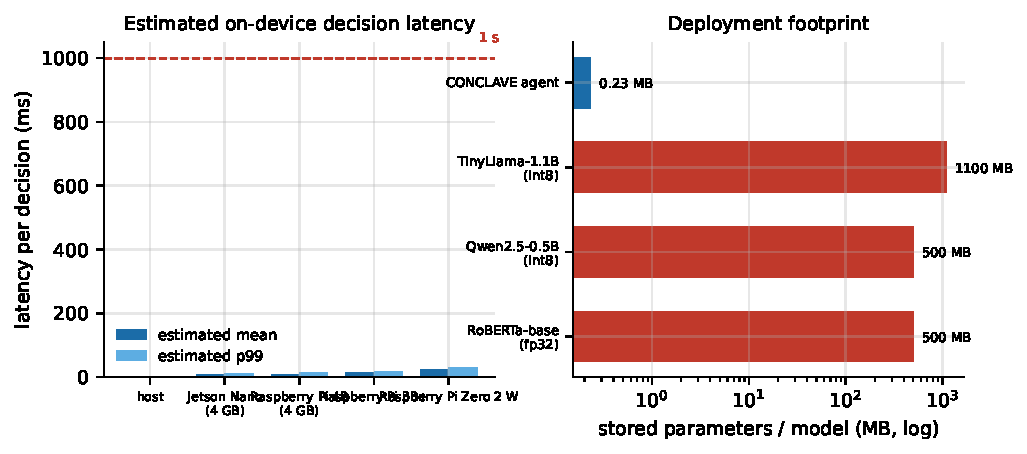
\includegraphics[width=\columnwidth]{fig4_edge.pdf}
\caption{Left: estimated per-decision latency across emulated boards, with the
1\,s mark shown for scale. Right: deployment footprint against the smallest
agent-capable language models, on a log axis.}
\label{fig:edge}
\end{figure}

The complete disaster agent --- featuriser and ensemble --- serialises to
$232$\,KB, roughly $2100\times$ smaller than a quantised 0.5B SLM's weights. Fig.~\ref{fig:edge} puts
that alongside the smallest language models the agentic literature considers.
Estimated decision latency is about $23$\,ms mean and $31$\,ms at the 99th percentile even on a Pi Zero
2\,W. We report one caveat plainly: peak resident memory is $217$\,MB, which is
dominated by the Python runtime and scientific stack, not the agent. On a
$512$\,MB board that fits, but a C or MicroPython deployment would remove most
of it, and we have not built one.

\subsection{Does the uncertainty signal earn its place?}
\begin{figure}[t]
\centering
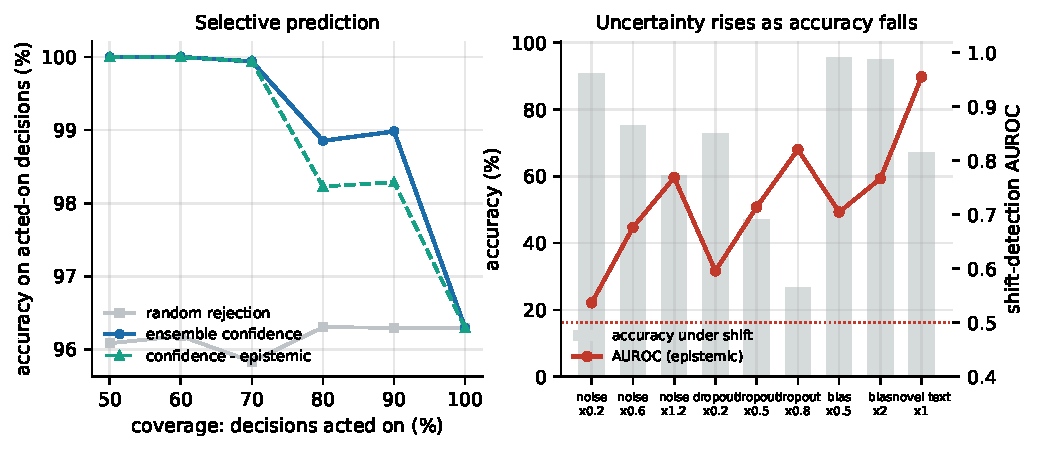
\includegraphics[width=\columnwidth]{fig3_uncertainty.pdf}
\caption{Left: selective prediction. Right: uncertainty tracks accuracy
degradation across covariate shifts.}
\label{fig:uncertainty}
\end{figure}

\textbf{Selective prediction works.} Accuracy on acted-on decisions rises from
$96.3\%$ at full coverage to $100\%$ at $50\%$ coverage, while random rejection
stays flat at $\sim\!96\%$ (AURC $0.946$).

\textbf{Shift detection works.} Across sensor noise, dropout, bias, and an
unfamiliar report vocabulary, uncertainty rises monotonically as accuracy falls
--- AUROC $0.955$ for novel text (accuracy $96.3\% \rightarrow 67.2\%$) and
$0.820$ for $80\%$ sensor dropout (accuracy $\rightarrow 26.6\%$). We note an
initial probe that shifted flood \emph{severity} gave AUROC $\approx 0.50$;
that was a flaw in the probe, not the signal, because the controller keeps
observations in-distribution under severity change. We report it because the
distinction --- shifting latent dynamics is not shifting covariates --- is easy
to get wrong.

\textbf{The decomposition does not beat plain confidence.} On both selective
prediction and shift detection, max-posterior confidence matches or slightly
exceeds the epistemic term (e.g.\ $0.960$ vs $0.955$ AUROC on novel text). The
theoretical appeal of separating aleatoric from epistemic uncertainty did not
translate into measured advantage on these tasks.

\textbf{And uncertainty-triggered oversight fails outright.} Under $60\%$
sensor dropout, with a budget of $10$ human interventions per episode, random
allocation lifts mean return from $-14.7$ to $+2.9$, while epistemic-triggered
allocation reaches only $-11.1$ and confidence-triggered $-10.3$. Random wins.
The diagnosis: instantaneous uncertainty is high in \emph{clusters}, so
uncertainty-triggered escalations bunch together early in an episode, whereas
random allocation spreads oversight across the horizon. In a sequential task,
\emph{when} a decision matters is at least as important as how uncertain it is,
and an instantaneous signal is blind to that. The correction is a
value-of-information criterion that weights uncertainty by the consequence of
error at that step; we have not implemented it, and we flag it as the most
promising direction for follow-up work.

\section{Discussion}

\subsection{When to use which core}
Our results do not show that ensemble agents are better than language-model
agents. They show the two occupy different regimes. A language model remains
necessary when the action space is open-ended, when the task specification
arrives in unconstrained natural language and changes between invocations, or
when the agent must compose genuinely novel plans. An ensemble core is
preferable when the tool set is enumerable, the observations are largely
structured, the decision recurs, the deployment is connectivity-denied or
power-constrained, or worst-case latency must be certified. Disaster response
sits squarely in the second regime, as do industrial monitoring, agricultural
control, and remote clinical triage.

\subsection{The cost of the language model was mostly not reasoning}
A striking implication of Section~\ref{sec:humaid} and Table~\ref{tab:routing}
is how much of an agentic pipeline turns out not to need language modelling.
Tool routing is ranking; abstention is binary classification; triage is
multi-class classification; sequential control is policy learning. The language
model in a conventional stack is doing work that is, for these tasks, largely
representational --- and a hashing featuriser plus a committee of small models
recovers most of that representation at a fraction of the cost.

\section{Limitations and Threats to Validity}
We state these plainly.

\textbf{No physical hardware.} We do not own a Raspberry Pi or Jetson board.
Core counts and RAM ceilings were genuinely enforced, but on-device latency and
energy are model-based estimates using literature-derived throughput ratios.
They should be treated as projections until measured on real boards.

\textbf{The sequential environment is a simulation.} Its dynamics are
hand-specified, and the expert controller that CONCLAVE clones is a heuristic
rather than an optimal policy. The availability result --- that a local brain
keeps working when the network does not --- is robust to these details, but
absolute returns are not meaningful outside the simulator.

\textbf{Argument filling is out of scope.} CONCLAVE routes to a tool and abstains
when none applies; it does not extract typed arguments from free text, which
BFCL's headline metric requires. Structured argument extraction with classical
methods is a real gap.

\textbf{The comparison to SLMs is on cost, not capability.} We did not run an
SLM baseline ourselves; we cite published numbers on a related but different
metric. A head-to-head evaluation on identical metrics and identical hardware
is the obvious next study.

\textbf{Text handling is lexical.} Hashed n-grams have no compositional
semantics. Negation, sarcasm, and paraphrase will hurt CONCLAVE more than a
transformer, which likely accounts for much of the HumAID gap.

\textbf{Peak memory is dominated by the runtime.} The agent is $232$\,KB; the
Python process is $217$\,MB. A genuinely microcontroller-class deployment needs
a reimplementation we have not attempted.

\section{Conclusion}
Agentic AI has converged on a single architectural assumption --- that a
language model belongs at the centre of the loop --- and that assumption
excludes exactly the deployments where autonomy has the highest stakes: the
flood district with no cell tower, the remote clinic on a solar panel. We built
CONCLAVE to test whether the assumption is load-bearing, and find that for
bounded, recurring, sensor-driven decision loops it largely is not. A
heterogeneous ensemble routes tools at $90.8\%$ top-1 accuracy in $4$\,ms from
$631$\,KB, triages crisis reports within $1.8$ F1 points of a transformer at
$1/14$ the size, and holds its performance flat while an oracle cloud agent
collapses as connectivity fails. It also has real limits, including one place
where our central intuition about uncertainty did not survive measurement.

The broader point is that ``agentic'' names a control architecture, not a model
class. Recovering that distinction makes autonomy available to a large class of
systems currently priced out of it.

\section*{Reproducibility}
All code, seeds, result artefacts, and figure-generation scripts are released
under Apache-2.0. Every result in this paper is regenerated by five scripts in
\texttt{experiments/}; each writes a JSON artefact recording platform, seed,
and commit. The full suite runs in under 30 minutes on the 2-core container
described in Section IV.

\balance
\bibliographystyle{IEEEtran}
\bibliography{references}

\end{document}
